\section{Experimental Evaluation}\label{Se:evaluation}

In this section, we describe quantiative results and share qualitative insight from our experimental evaluation of \Tool. 

\subsection{Experimental Setup and Methodology}

For our experiments, we assembled a suite of 80 Android apps: 4 enterprise apps, 3 apps shipping with version 4.4 of the Android platform as well as the 73 top-popular Google Play apps in the geography of one of the authors.
The experiments were conducted atop a Samsung Nexus 5 device running version 4.4 of the Android platform (CyanogenMod 11). For accuracy and reproducibility, we reset the device to a clean image before testing each of the apps.

Prior to running \Tool, a professional ethical hacker audited all 80 apps. The audit resulted in a total of 80 IAC vulnerabilities (per the catalog in \secref{attackSurface}). These are listed in \tableref{vulns}.

\subsection{Quantitative Evaluation}

We have conducted a series of experiments to measure, and thereby justify, the key features of \Tool. We organize our description of the experiments around four research hypotheses. The starting point is a baseline algorithm that only targets the {\tt data} field of {\tt Intent} objects built according to the declared IAC interface.

\paragraph{H1: Probing Boosts Performance} To quantify the performance gain thanks to probing, we enhanced the baseline algorithm with necessary-conditions specifications as described in \secref{detectionSubsec}. Instead of blindly attempting all possible test payloads, the enhanced version first analyzes the probing trace to focus testing only on relevant attack types.

The statistics demonstrate significant improvement. While naive fuzzing expends an average of 64 tests and 24 minutes per app, the enhanced version requires $<15$ tests and $<7$ minutes per app to detect the same set of IAC vulnerabilities.

\paragraph{H2: String Extras are Often Vulnerable} The naive testing algorithm, equipped with probing capabilities, is able to detect a total of 94 out of the 165 known vulnerabilities for a recall rate of $<0.57$. Enhancing it to incorporate string extras as attack targets pushes recall up to 0.85, as 46 new vulnerabilities are detected.

The resulting variant has an iterative testing loop, which attacks targets discovered in previous probing/testing rounds. Naturally, this renders it more expensive than its naive counterpart with an average of 26 (compared to 15) tests and 12 (compared to 7) minutes per app.

\paragraph{H3: Boolean Extras Manifest in Path Conditions} The algorithm featuring both probing and manipulation of string extras already detects 140 out of the 165 known vulnerabilities. A natural means to increase coverage further is by exploring new execution paths.

Augmenting the testing algorithm to explore different combinations of boolean extras achieves this goal effectively. This is seen through the discovery of 11 new vulnerabilities, constituting a 7\% improvement in recall, for a total of 151 vulnerabilities detected fully automatically. 

The cost, as expected, is also noticeable. The average number of tests per app climbs from 26 to 63 (x2.42 more tests) with a proportional rise in testing time from 12 to 25 minutes (x2.1 more time). This motivates a more effective algorithm to detect new paths.

\paragraph{H4: Linear-time Path Exploration is Effective} The fourth and final hypothesis concerns the relationship between boolean extras in their capacity as branching expressions. The claim is that it is effective to treat boolean extras as either dominating each other or being independent.

Under this assumption, which enables toggling of boolean extras one at a time and thus linear-complexity path exploration, testing time drops to 19 minutes (24\% improvement) and the average number of tests is only 40 compared to 63 before (37\% improvement). At the same time, only one of the 151 vulnerabilities detected via the exponential-time path-exploration algorithm is missed for a negligible drop of $<1$\% in recall.

\paragraph{Discussion} As we demonstrate via experimental validation of the four hypotheses above, \Tool\ embodies effective features to balance performance against coverage.\footnote{
	Beyond the data we present here, which confirms our design choices as a series of enhancements, we have a full matrix of measurements per every combination of the choices we've made. We have omitted most of these measurements for lack of space, but note that they are in strong support of our hypotheses.
} A visual illustration of the performance/coverage tradeoffs achieved by the different variants is provided in \figref{trends}. \Tool\ is denoted there as ``Linear PC''.

\figref{trends} highlights ``String Extras'' as the variant that maximizes the recall/performance gap. Even though the increase in performance exceeds the gain in coverage when switching to ``Linear PC'', we still view this option as more preferable, as less true warnings are missed in return for affordable performance slowdown.

\begin{figure}
	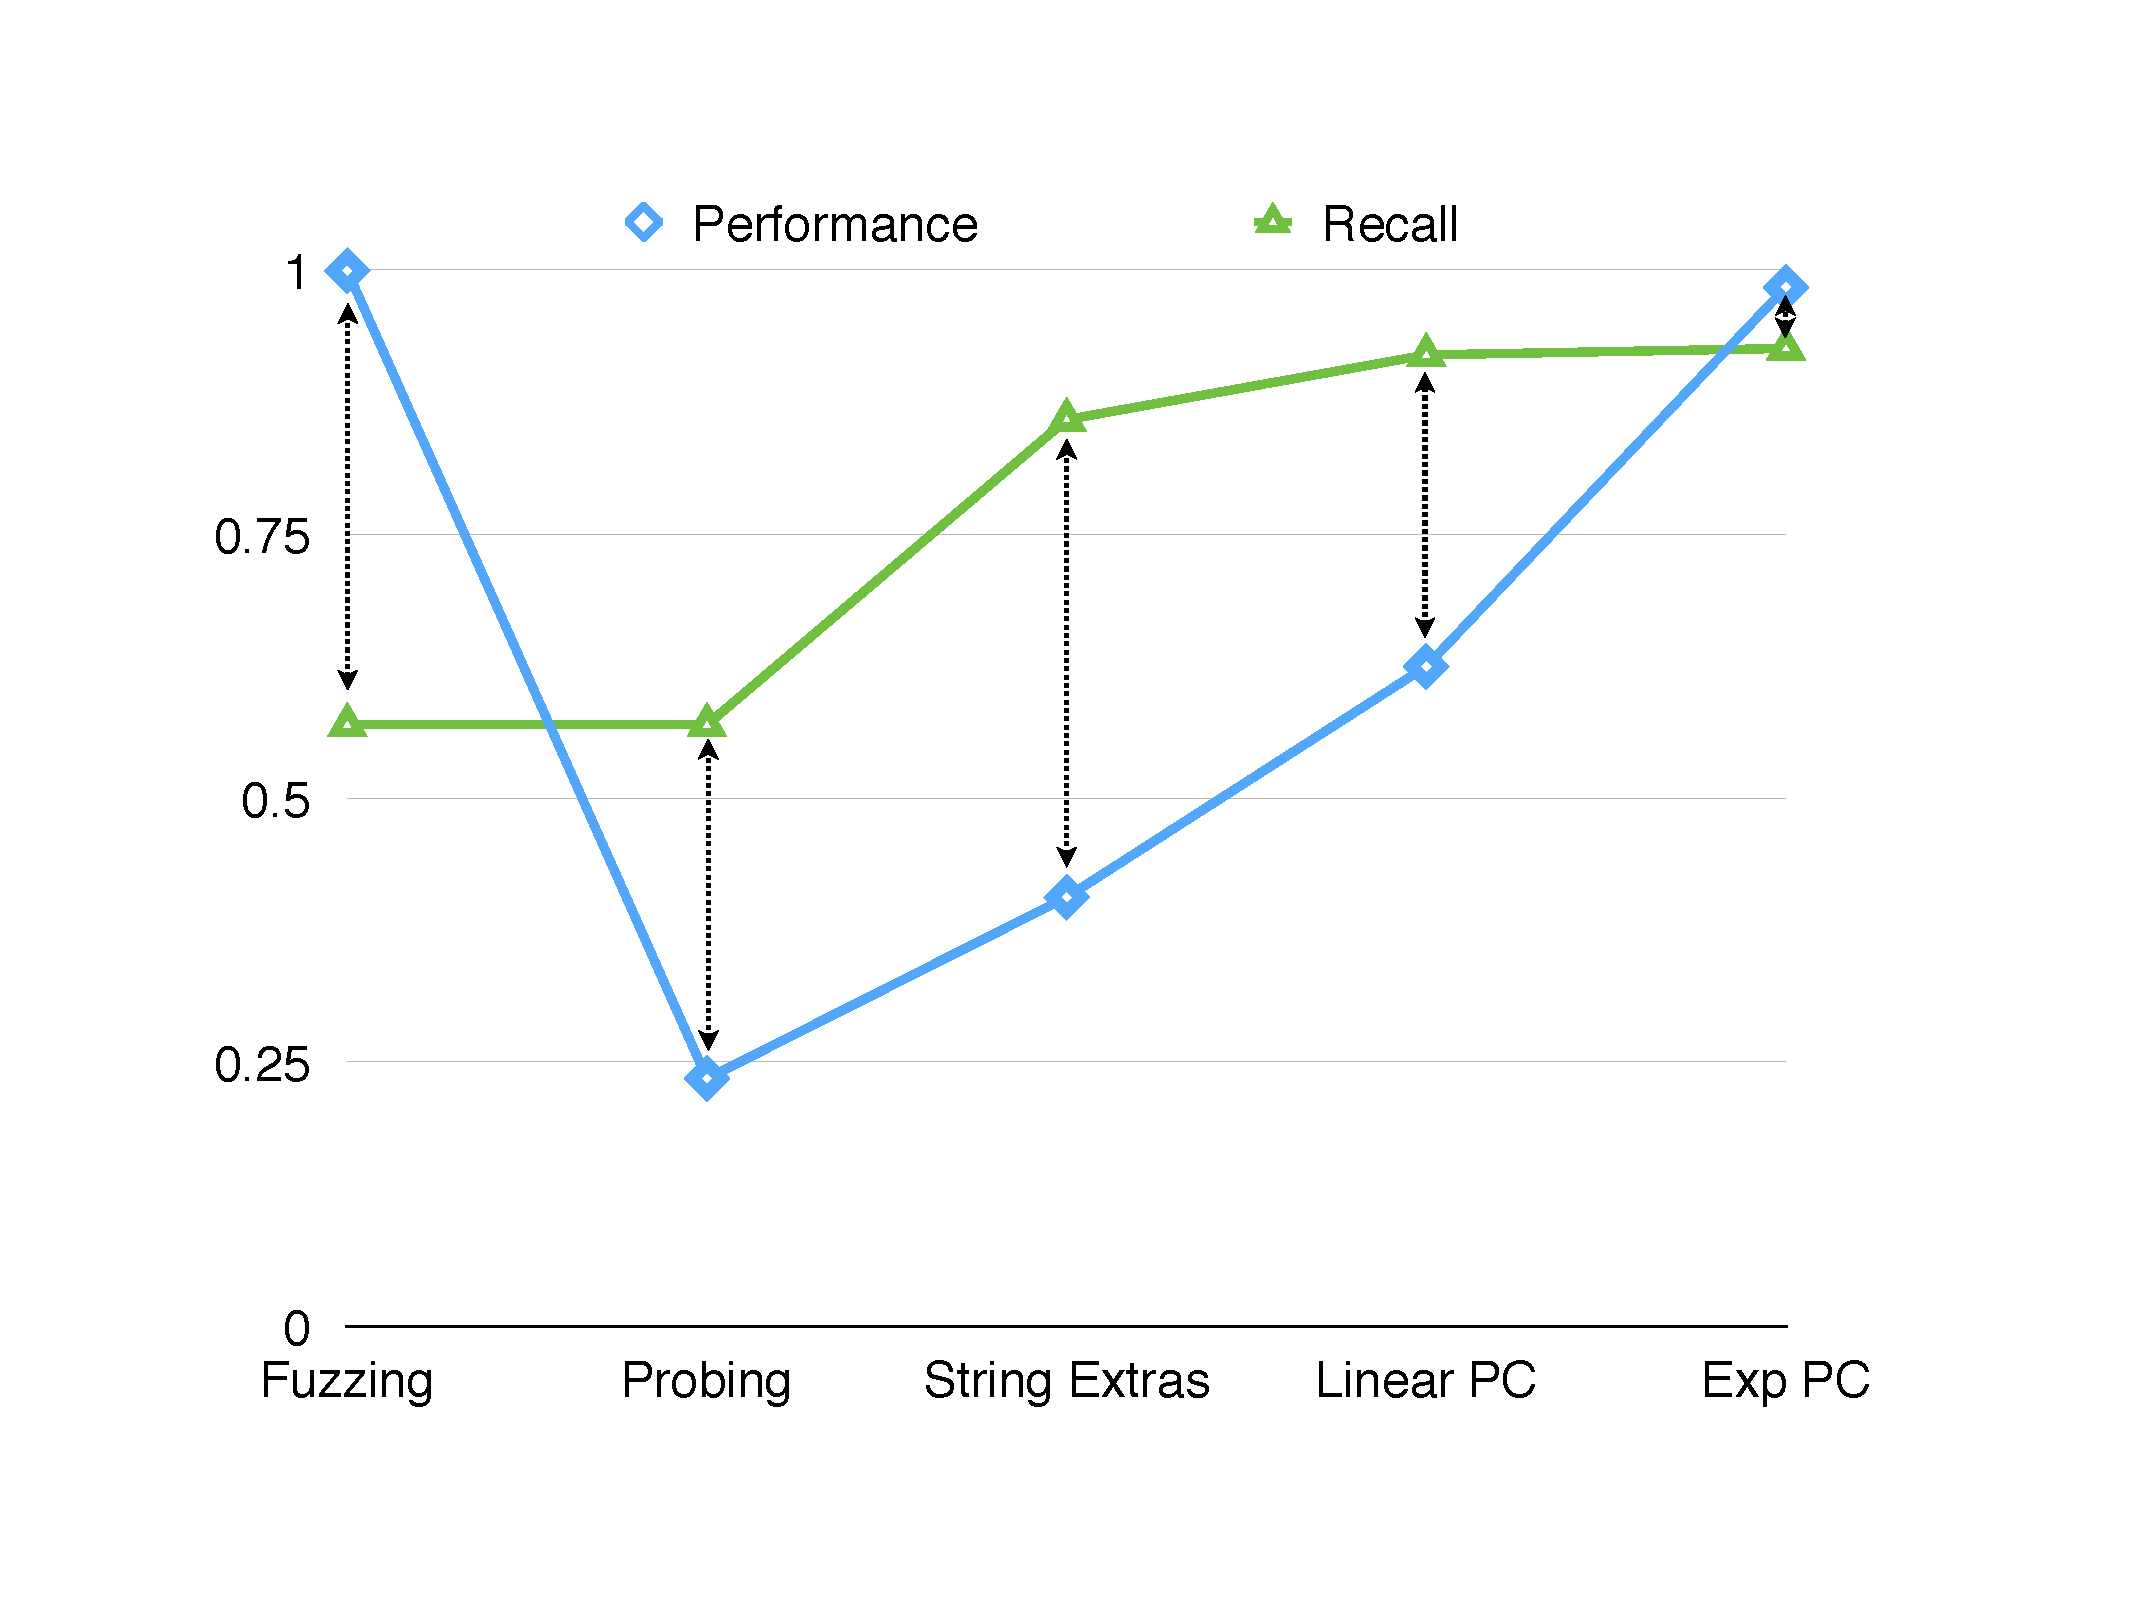
\includegraphics[width=\columnwidth]{trendline.pdf}
	\caption{\label{Fi:trends}Visual Performance/Recall Comparison between Testing Variants}
\end{figure}

%\subsection{H1: IAC Vulnerabilities are Prevalent}
%
%The first and foremost hypothesis guiding this research is that Android IAC is the cause of many security vulnerabilities in real-world apps:
%\begin{quote}
%	\emph{H1: On average, a real-world Android app suffers from at least one security vulnerability due to improper handling of incoming IAC data.}
%\end{quote}
%To test this hypothesis, we thoroughly studied all 80 of our benchmark apps as follows:
%\begin{enumerate}
%	\item We applied bound-free fuzz testing to all the apps, having the fuzzing tool fire payloads at the app with unlimited testing budget. The fuzzing tool is obtained by disabling all the detection heuristics, performance optimizations and testing bounds implemented in \Tool. This leads to testing of all possible input points (including those failing the detection stage), manipulation of all boolean extras, etc.
%	\item We additionally applied manual analysis to some of the apps: both (i) interactive debugging and (ii) decompilation of the app and inspection of its source code.
%\end{enumerate}
%
%The results we obtained are summarized in \tableref{vulns}. We present the findings for apps in which we discovered at least one vulnerability. There are 52 such apps, which comprise 65\% of the benchmarks in our suite. For each of the vulnerable apps, we present both (i) the total number of detected vulnerabilities and (ii) a breakdown of the vulnerabilities into categories, which reflects the vulnerability types the app suffers from. (See \secref{attackSurface}.)

\begin{table*}
\begin{scriptsize}
\begin{center}
\begin{tabular}{l|c|c|c|c|c|c|c|c|c}
\multicolumn{1}{c|}{\multirow{2}{*}{App Name}} & \multirow{2}{*}{Count} & \multirow{2}{*}{XAS} & \multirow{2}{*}{SQLi} & Unsafe  & UI  & {\tt Fragment}  & Java  & Native  & File  \\
 &  &  &  &  Reflection &  Spoofing &  Injection &  Crash &  Crash &  Manipulation \\
\hline
\_Dropbox v2.3.8 & 4 & \xmark & \xmark & \xmark & \xmark & \cmark & \cmark & \xmark & \xmark \\
\_eBay v2.3.0.25 & 3 & \xmark & \xmark & \cmark & \xmark & \xmark & \cmark & \xmark & \xmark \\
\_Evernote v5.1.2 & 7 & \xmark & \xmark & \xmark & \xmark & \cmark & \cmark & \xmark & \xmark \\
\_Facebook v3.3 & 4 & \xmark & \xmark & \xmark & \xmark & \xmark & \cmark & \xmark & \xmark \\
\_Gmail v4.5-836823 & 2 & \xmark & \xmark & \xmark & \xmark & \cmark & \cmark & \xmark & \xmark \\
\_IBM Notes Traveler v9.0.0.0 201306202317 & 1 & \xmark & \xmark & \xmark & \xmark & \xmark & \cmark & \xmark & \xmark \\
\_LinkedIn v3.0.2 & 6 & \xmark & \xmark & \xmark & \xmark & \xmark & \cmark & \xmark & \xmark \\
\_NYTimes for Android v3.2.2 & 2 & \cmark & \xmark & \xmark & \xmark & \xmark & \cmark & \xmark & \xmark \\
\_YouTube v4.5.17 & 2 & \xmark & \xmark & \xmark & \xmark & \xmark & \cmark & \xmark & \xmark \\
Adobe Reader v10.6.0 & 3 & \xmark & \xmark & \xmark & \xmark & \xmark & \cmark & \xmark & \xmark \\
Chrome Browser - Google v27.0.1453.90 & 1 & \xmark & \xmark & \xmark & \xmark & \xmark & \cmark & \xmark & \xmark \\
com.alibaba.aliexpresshd-1. & 1 & \xmark & \xmark & \xmark & \xmark & \xmark & \cmark & \xmark & \xmark \\
com.android.vending-1 & 3 & \xmark & \xmark & \xmark & \xmark & \cmark & \cmark & \xmark & \xmark \\
com.box.android-1. & 1 & \xmark & \xmark & \xmark & \xmark & \xmark & \cmark & \xmark & \xmark \\
com.fitbit.FitbitMobile-1. & 1 & \xmark & \xmark & \xmark & \xmark & \xmark & \cmark & \xmark & \xmark \\
com.google.android.apps.docs.editors.sheets-1. & 4 & \xmark & \xmark & \xmark & \xmark & \xmark & \cmark & \xmark & \xmark \\
com.google.android.apps.maps-1. & 2 & \xmark & \xmark & \xmark & \xmark & \xmark & \cmark & \xmark & \xmark \\
com.google.android.maps.mytracks-1. & 3 & \xmark & \xmark & \xmark & \cmark & \xmark & \cmark & \xmark & \xmark \\
com.google.android.music-1. & 4 & \xmark & \xmark & \xmark & \xmark & \xmark & \cmark & \xmark & \xmark \\
com.google.android.talk-2. & 1 & \xmark & \cmark & \xmark & \xmark & \xmark & \xmark & \xmark & \xmark \\
com.google.earth-1. & 1 & \xmark & \xmark & \xmark & \xmark & \xmark & \cmark & \xmark & \xmark \\
com.ideomobile.hapoalim-1. & 12 & \cmark & \xmark & \xmark & \cmark & \xmark & \cmark & \xmark & \xmark \\
com.ideomobile.leumicard-1 & 2 & \cmark & \xmark & \xmark & \xmark & \xmark & \cmark & \xmark & \xmark \\
com.intsig.camscanner-1. & 1 & \xmark & \xmark & \xmark & \xmark & \xmark & \cmark & \xmark & \xmark \\
com.leumi.leumiwallet-1. & 1 & \xmark & \xmark & \xmark & \xmark & \xmark & \cmark & \xmark & \xmark \\
com.melodis.midomiMusicIdentifier.freemium-1. & 2 & \cmark & \xmark & \xmark & \xmark & \xmark & \cmark & \xmark & \xmark \\
com.mxtech.videoplayer.ad-1. & 2 & \xmark & \xmark & \xmark & \xmark & \cmark & \cmark & \xmark & \xmark \\
com.paypal.android.p2pmobile-1 & 1 & \xmark & \xmark & \xmark & \xmark & \xmark & \cmark & \xmark & \xmark \\
com.runtastic.android-1. & 1 & \xmark & \xmark & \xmark & \xmark & \xmark & \cmark & \xmark & \xmark \\
com.urbandroid.sleep-1. & 4 & \xmark & \xmark & \xmark & \xmark & \cmark & \cmark & \xmark & \xmark \\
com.viber.voip-1. & 2 & \xmark & \xmark & \xmark & \xmark & \xmark & \cmark & \xmark & \xmark \\
com.waze-1. & 1 & \xmark & \xmark & \xmark & \xmark & \xmark & \cmark & \xmark & \xmark \\
com.yelp.android-1. & 4 & \xmark & \xmark & \xmark & \xmark & \xmark & \cmark & \xmark & \xmark \\
Contacts. & 7 & \xmark & \xmark & \xmark & \cmark & \xmark & \cmark & \xmark & \xmark \\
Dialer. & 2 & \xmark & \xmark & \xmark & \xmark & \xmark & \cmark & \xmark & \xmark \\
Facebook Messenger v2.5.3-release & 1 & \xmark & \xmark & \cmark & \xmark & \xmark & \xmark & \xmark & \xmark \\
Facebook Pages Manager v1.4.1 & 1 & \xmark & \xmark & \cmark & \xmark & \xmark & \xmark & \xmark & \xmark \\
mobi.mgeek.TunnyBrowser-1. & 1 & \xmark & \xmark & \xmark & \xmark & \xmark & \cmark & \xmark & \xmark \\
org.zwanoo.android.speedtest-1 & 1 & \xmark & \xmark & \xmark & \xmark & \xmark & \cmark & \xmark & \xmark \\
Shazam v3.14.0-JB78059 & 5 & \cmark & \xmark & \xmark & \xmark & \xmark & \cmark & \xmark & \xmark \\
Tango Text Voice and Video v2.10.48610 & 3 & \xmark & \xmark & \xmark & \xmark & \xmark & \cmark & \xmark & \xmark \\
Firefox Browser for Android v22.0 & 6 & \xmark & \xmark & \xmark & \cmark & \xmark & \cmark & \xmark & \cmark \\
GO Launcher EX v3.9.11 & 2 & \xmark & \xmark & \xmark & \xmark & \xmark & \cmark & \xmark & \xmark \\
Google Drive v1.2.182.26 & 5 & \xmark & \xmark & \xmark & \cmark & \xmark & \cmark & \xmark & \xmark \\
Google Finance v2.2.7 & 2 & \xmark & \xmark & \xmark & \xmark & \xmark & \cmark & \xmark & \xmark \\
Google Translate v2.7 & 2 & \xmark & \xmark & \cmark & \xmark & \xmark & \cmark & \xmark & \xmark \\
GTasks v1.6.0.2 & 11 & \xmark & \xmark & \xmark & \xmark & \cmark & \cmark & \xmark & \xmark \\
IBM Connections v4.4.0 & 5 & \xmark & \xmark & \xmark & \xmark & \xmark & \cmark & \xmark & \xmark \\
IBM Sametime Meetings v8.5.2.4 & 3 & \xmark & \xmark & \xmark & \xmark & \xmark & \cmark & \xmark & \xmark \\
IBM Sametime v8.5.2.4 201304171550 & 1 & \xmark & \xmark & \xmark & \xmark & \xmark & \cmark & \xmark & \xmark \\
Instagram v3.5.3 & 3 & \xmark & \xmark & \xmark & \xmark & \xmark & \cmark & \xmark & \xmark \\
Mms & 3 & \xmark & \xmark & \xmark & \cmark & \xmark & \cmark & \xmark & \xmark \\
\hline\hline
\multicolumn{1}{c|}{{\bf 52/80}} & {\bf 165} & {\bf 5} & {\bf 1} & {\bf 4}  & {\bf 6}  & {\bf 7} & {\bf 50} & {\bf 0} & {\bf 1} \\
\end{tabular}
\end{center}
\end{scriptsize}
\caption{\label{Ta:vulns}Detected Vulnerabilities with Breakdown by Attack Type}
\end{table*}

%The data from our study provides firm evidence in favor of hypothesis H1: The majority of apps in our suite (65\%) exhibit IAC vulnerabilities with a total of 165 vulnerabilities across 52 apps. That is, on average a vulnerable app suffers from roughly 3 IAC vulnerabilities (165/52), and an app in general suffers from roughly 2 IAC vulnerabilities (165/80). 
%
%The most common type of vulnerability, by far, is crashes due to improper handling of IAC data. This is consistent with the empirical data reported by Maji et al. \cite{MAB:DSN12}. IAC-induced crashes expose the app to denial-of-service attacks as well as information theft. Classic injection vulnerabilities --- in the form of XAS, SQLi, unsafe reflection and file manipulation --- exist in 12 of the benchmark apps, which is $>$10\% of all apps and $>$20\% of the vulnerable apps in our suitem. 13 of the apps suffer from Android-specific injection vulnerabilities: {\tt Fragment} injection and UI spoofing. Finally, for the threat of native crash (exemplified in \figref{techExample}), we could not find any app suffering from this weakness. This suggests that native APIs (like {\tt NativeIO.write($\ldots$)}) are not in frequent use, let alone driven by user input.
%
%\subsection{H2: Naive Fuzz Testing Is Ineffective at Detecting IAC Vulnerabilities}
%
%Having established the prevalence of IAC-related vulnerabilities, we validate through our second hypothesis that simply bombarding IAC input points with security payloads is not satisfactory, as the cost paid in performance yields only few additional findings beyond the testing strategy of \Tool:
%\begin{quote}
%	\emph{H2: Fuzz testing strikes an undesirable tradeoff between performance and detected vulnerabilities, suggesting that detection-based testing is needed.}
%\end{quote}
%To check into this hypothesis, we disabled the \Tool\ detection step. In the resulting configuration, attacks are fired blindly at publicly known as well as dynamically discovered input points.   
%%
%\tableref{FuzzVsTool} compares the results obtained by running brute-force fuzzing compared to \Tool\ against our suite of 80 benchmark applications.  The comparison focuses on running time, number of tests executed and total number of vulnerabilities detected. 
%
%\begin{table*}
%\begin{scriptsize}
%\begin{center}
%\begin{tabular}{l|c|c|c|c|c|c}
%\multicolumn{1}{c|}{\multirow{2}{*}{App Name}} & \multicolumn{3}{c|}{Fuzzing} &  \multicolumn{3}{c}{\Tool}  \\
%\cline{2-7}
%&  Time (m) &  Tests &  Vulnerabilities &  Time (m) &  Tests &  Vulnerabilities \\ \hline
%com.yahoo.mobile.client.android.flickr-1. & 34 & 6 & 0 & 7 & 3 & 0 \\
%com.waze-1. & 14 & 2 & 1 & 4 & 1 & 1 \\ 
%com.google.android.apps.docs.editors.sheets-1. & 274 & 96 & 4 & 72 & 28 & 4 \\ 
%com.fibi-1 & 7 & 0 & 0 & 1 & 0 & 0 \\ 
%Skype - free IM and video calls v3.2.0.6673 & 91 & 8 & 0 & 13 & 2 & 0 \\ 
%Dialer. & 130 & 18 & 2 & 35 & 14 & 2 \\ 
%TED v1.1.6 & 20 & 1 & 0 & 3 & 0 & 1 \\ 
%Antivirus Security - FREE v3.2.3 & 13 & 1 & 0 & 2 & 0 & 0 \\ 
%com.snapchat.android-1. & 7 & 1 & 0 & 1 & 0 & 0 \\ 
%com.google.android.apps.maps-1. & 70 & 33 & 2 & 11 & 7 & 2 \\ 
%com.google.android.apps.plus-1. & 1930 & 500 & 10 & 446 & 164 & 12 \\ 
%com.intsig.camscanner-1. & 307 & 138 & 1 & 55 & 40 & 0 \\ 
%com.google.android.talk-2. & 1344 & 726 & 1 & 54 & 35 & 0 \\ 
%org.telegram.messenger-1. & 28 & 15 & 0 & 4 & 2 & 0 \\ 
%Facebook Messenger v2.5.3-release & 66 & 49 & 1 & 37 & 32 & 1 \\ 
%GO Launcher EX v3.9.11 & 183 & 24 & 2 & 28 & 10 & 3 \\ 
%Shazam v3.14.0-JB78059 & 416 & 179 & 5 & 112 & 49 & 5 \\ 
%Google Finance v2.2.7 & 34 & 23 & 2 & 7 & 4 & 2 \\ 
%com.alibaba.aliexpresshd-1. & 47 & 6 & 1 & 9 & 2 & 1 \\ 
%com.paypal.android.p2pmobile-1 & 446 & 174 & 1 & 63 & 43 & 1 \\ 
%Google Currents v2.1.0 & 61 & 23 & 0 & 18 & 6 & 0 \\ 
%com.google.android.apps.magazines-1. & 20 & 4 & 0 & 6 & 2 & 0 \\ 
%IBM SmartCloud Meetings v8.5.2.1.201212060646 & 14 & 10 & 0 & 2 & 1 & 0 \\ 
%com.nike.plusgps-1. & 7 & 4 & 0 & 1 & 1 & 0 \\ 
%com.google.android.music-1. & 303 & 154 & 4 & 13 & 12 & 1 \\ 
%\_NYTimes for Android v3.2.2 & 54 & 8 & 2 & 11 & 2 & 2 \\ 
%IBM Connections v4.4.0 & 455 & 147 & 5 & 313 & 203 & 5 \\ 
%Mms & 433 & 104 & 3 & 74 & 25 & 3 \\ 
%com.ubercab-1. & 28 & 10 & 0 & 12 & 3 & 0 \\ 
%Adobe Reader v10.6.0 & 34 & 4 & 3 & 9 & 1 & 3 \\ 
%GTasks v1.6.0.2 & 557 & 260 & 11 & 123 & 50 & 11 \\ 
%IBM Sametime v8.5.2.4 201304171550 & 34 & 11 & 1 & 9 & 3 & 1 \\ 
%Google Translate v2.7 & 95 & 24 & 2 & 22 & 9 & 1 \\ 
%Adobe Photoshop Express v1.3.3 & 21 & 1 & 0 & 5 & 0 & 0 \\ 
%com.ideomobile.hapoalim-1. & 708 & 339 & 12 & 124 & 76 & 12 \\ 
%WhatsApp Messenger v2.10.222 & 84 & 62 & 0 & 12 & 7 & 0 \\ 
%com.google.android.maps.mytracks-1. & 55 & 37 & 3 & 13 & 8 & 3 \\ 
%org.zwanoo.android.speedtest-1 & 21 & 3 & 1 & 3 & 1 & 1 \\ 
%com.urbandroid.sleep-1. & 249 & 47 & 4 & 44 & 12 & 4 \\ 
%com.viber.voip-1. & 335 & 70 & 2 & 40 & 21 & 2 \\ 
%com.runtastic.android-1. & 56 & 16 & 1 & 13 & 7 & 1 \\ 
%Facebook Pages Manager v1.4.1 & 32 & 16 & 1 & 8 & 7 & 1 \\ 
%com.google.android.GoogleCamera-1 & 63 & 7 & 0 & 8 & 2 & 0 \\ 
%com.google.android.apps.m4b-1. & 14 & 3 & 0 & 2 & 1 & 0 \\ 
%com.hipmunk.android-1. & 7 & 3 & 0 & 1 & 0 & 0 \\ 
%Contacts. & 323 & 92 & 7 & 99 & 50 & 7 \\ 
%com.cleanmaster.security-1. & 53 & 15 & 0 & 6 & 3 & 0 \\ 
%Chrome Browser - Google v27.0.1453.90 & 112 & 12 & 3 & 66 & 10 & 1 \\ 
%\_Gmail v4.5-836823 & 348 & 82 & 2 & 100 & 35 & 2 \\ 
%IBM Sametime Meetings v8.5.2.4 & 21 & 2 & 3 & 5 & 0 & 2 \\ 
%Tiny Flashlight + LED v4.9.4 & 28 & 16 & 0 & 4 & 3 & 0 \\ 
%com.ideomobile.leumicard-1 & 167 & 37 & 2 & 34 & 17 & 2 \\ 
%\_YouTube v4.5.17 & 473 & 141 & 2 & 42 & 21 & 0 \\ 
%com.box.android-1. & 166 & 107 & 1 & 26 & 19 & 1 \\ 
%Firefox Browser for Android v22.0 & 277 & 74 & 6 & 71 & 25 & 5 \\ 
%\_Facebook v3.3 & 1861 & 1947 & 4 & 24 & 27 & 1 \\ 
%com.netgate-1 & 14 & 5 & 0 & 4 & 2 & 0 \\ 
%Instagram v3.5.3 & 42 & 8 & 3 & 9 & 3 & 2 \\ 
%clalit.android-1. & 40 & 5 & 0 & 6 & 3 & 0 \\ 
%Tango Text Voice and Video v2.10.48610 & 48 & 6 & 3 & 7 & 1 & 3 \\ 
%com.yelp.android-1. & 147 & 68 & 4 & 34 & 26 & 3 \\ 
%com.google.earth-1. & 48 & 5 & 1 & 21 & 3 & 1 \\ 
%\_LinkedIn v3.0.2 & 763 & 345 & 6 & 166 & 104 & 6 \\ 
%Google Drive v1.2.182.26 & 370 & 131 & 5 & 94 & 42 & 5 \\ 
%com.mxtech.videoplayer.ad-1. & 199 & 36 & 2 & 100 & 22 & 1 \\ 
%Adobe AIR v3.7.0.209 & 21 & 1 & 0 & 3 & 3 & 0 \\ 
%XBMC remote control v2.0.1 & 7 & 0 & 0 & 1 & 0 & 0 \\ 
%\_eBay v2.3.0.25 & 201 & 60 & 3 & 32 & 18 & 2 \\ 
%IMDB Movies And TV v3.2.2.103220310 & 40 & 32 & 0 & 7 & 6 & 0 \\ 
%\_Dropbox v2.3.8 & 265 & 111 & 4 & 67 & 32 & 4 \\ 
%com.android.vending-1 & 228 & 82 & 3 & 35 & 17 & 3 \\ 
%com.fitnesskeeper.runkeeper.pro-1. & 166 & 86 & 0 & 14 & 9 & 0 \\ 
%com.leumi.leumiwallet-1. & 20 & 2 & 1 & 5 & 1 & 1 \\ 
%com.melodis.midomiMusicIdentifier.freemium-1. & 83 & 72 & 2 & 16 & 11 & 2 \\ 
%\_Evernote v5.1.2 & 706 & 331 & 7 & 126 & 71 & 7 \\ 
%mobi.mgeek.TunnyBrowser-1. & 263 & 44 & 1 & 70 & 30 & 1 \\ 
%com.onoapps.cal4u-1 & 7 & 0 & 0 & 1 & 0 & 0 \\ 
%\_IBM Notes Traveler v9.0.0.0 201306202317 & 133 & 36 & 1 & 24 & 12 & 1 \\ 
%com.fitbit.FitbitMobile-1. & 14 & 5 & 1 & 2 & 1 & 1 \\ 
%Opera browser beta v15.0.1162.59192 & 35 & 2 & 0 & 5 & 1 & 0 \\
%\hline\hline
%\multicolumn{1}{c|}{{\bf 80}} & {\bf 211} & {\bf 92} & {\bf 165} & {\bf 40}  & {\bf 19}  & {\bf 150}  \\
%\end{tabular}
%\end{center}
%\end{scriptsize}
%\caption{\label{Ta:FuzzVsTool}Comparison between Fuzzing and \Tool}
%\end{table*}
%
% The data in \tableref{FuzzVsTool} confirms hypothesis H2: On average, \Tool\ is $81.2\%$ faster and executes $79.3\%$ fewer tests than brute-force fuzzing. Fuzz testing requires over an hour and half on average for a single app, whereas \Tool\ completes a scan in under 20 minutes. This is a dramatic difference. Though completeness takes precedence over performance, we do not view an average scanning time of 92 minutes as acceptable.
% As for completeness, \Tool\ fails to detect only 9\% of the vulnerabilities discovered via fuzz testing. Out of 165 vulnerabilities reported in total by the fuzzing tool, \Tool\ is able to detect 150.
%
%\subsection{H3: Vulnerabilities Involving Extra Parameters are Prevalent}
%
%A powerful feature of \Tool\ is its iterative testing algorithm, described in \secref{corealg} (and in specific in \secref{iterative}), which incrementally uncovers and tests implicit IAC input points in the form of extra parameters. The third hypothesis we evaluated concerns the efficacy of this feature:
%\begin{quote}
%	\emph{H3: The increase in detected vulnerabilities thanks to targeting of extra parameters is significant compared to the baseline of testing only declared input points.}
%\end{quote}
%To assert whether this is indeed the case, we created a configuration of \Tool\ wherein extra parameters (both strings and booleans) are fully ignored. We refer to this configuration in \tableref{booleanExtras} as ``None''. Comparatively, the ``Exponential'' strategy is the most comprehensive testing strategy that can be implemented on top of the core \Tool\ algorithm. In this configuration, \Tool\ records and tests all string extras. Also, \Tool\ explores all possible combinations of boolean extras to maximize coverage.
%
%The gap between the ``None'' and ``Exponential'' configurations in detected vulnerabilities reflects the relative weight of the implicit interface in the overall coverage achieved by \Tool. Under ``Exponential'', \Tool\ detects 151 distinct vulnerabilities compared to only 94 vulnerabilities under ``None''. This constitutes a reduction of approximately 38\% in detected vulnerabilities. That is, over $\sfrac{1}{3}$ of the detected vulnerabilities require manipulation of extra parameters. Boolean extras reveal more app behaviors (by toggling the values of boolean flags), and string extras are direct attack targets.
%
%To distinguish the contribution of the two extra types to overall detection of vulnerabilities, we refer to a third configuration, ``Naive'', that records and tests string extras while completely disregarding boolean extras. That is, vulnerabilities that can only be discovered by exploring non-default combinations of boolean-extra flags are missed by ``Naive''. The data in \tableref{booleanExtras} suggests that most, though not all, of the vulnerabilities are still detectable: 140 out of the 151 issues reported by ``Exponential'' are also reported by ``Naive''. 
%
%This suggests that string extras outweigh boolean extras in importance in security testing. Our analysis of the data supporting this conclusion has led us to hypothesize that even though boolean extras contribute to coverage, different paths through the code often ultimately converge at mutual security-sensitive operations. Therefore, even though coverage is hindered, many of the vulnerabilities can still be detected without switching boolean extras away from their default values. Still, over 7\% of the vulnerabilities are missed in this setting, which is dramatic given the severity of IAC vulnerabilities.
%
%Another summarized view of the data in \tableref{booleanExtras} is obtained by quantifying the empirical likelihood of an extra parameter being vulnerable in comparison with the data field. To estimate this quantity, we compute the following measures:
%\begin{itemize}
%	\item The average number of vulnerabilities per the data field, {\tt uri}, is computed as the total number of vulnerabilities reported by the ``None'' configuration divided by the total number of test payloads sent under this configuration. Note that this is not a precise measure, as path conditions governed by boolean extras that can potentially lead to the detection of additional vulnerabilities are not explored. Still, this is a useful approximation.
%	\item For the likelihood of a vulnerability with respect to a string-extra field, we consider the difference between the ``Exponential'' and ``Naive'' configurations. We compute the same ratio as before (i.e., number of vulnerabilities divided by number of tests), but calculate both as the difference between the two configurations.
%	\item Finally, to quantify the likelihood of a vulnerability involving extras in general (both booleans and strings), we compute the same ratio as in the two previous cases, but this time the difference we calculate is between ``Exponential'' and ``None''. The delta in this case is between full manipulation of both types of extras and completely ignoring both.
%\end{itemize}
%
%The results of the calculations described above are as follows:
%\begin{center}
%	\begin{tabular}{l|ccc}
%									& {\it data field} & {\it string extras} & {\it all extras} \\
%									\hline
%		{\it tests} 	 				&  1612       & 2294 &  2976 \\
%		{\it vulnerabilities}  	& 140	     & 11 & 57 \\
%		\hline\hline
%		{\it likelihood} & 0.09 & 0.005 & 0.02 \\
%	\end{tabular}
%\end{center}
%These statistics indicate that, by far, the most likely target for an IAC attack is the {\tt uri} field. At the same time, manipulating both string and boolean extras simultaneously results in a vulnerability in approximately one out of 50 tests. The average drops sharply if only string extras are manipulated. In this case, only one of out 2000 tests would detect a problem. The conclusion, in light of this analysis, is that \Tool\ is justified in targeting both types of extra parameters in addition to the data field.
%
%%\begin{table}
%%\begin{small}
%%\begin{center}
%%\begin{tabular}{l|c|c}
%%\multirow{2}{*}{App Name} & \multicolumn{2}{c}{Vulnerabilities}  \\
%%\cline{2-3}
%%		&  w. Extras & w.o. Extras \\
%%\hline
%%Aaaaa & 10 & 6 \\
%%\end{tabular}
%%\end{center}
%%\end{small}
%%\caption{\label{Ta:stringExtras}Effect of attacking string extras}
%%\end{table}
%
%\begin{table*}
%\begin{scriptsize}
%\begin{center}
%\begin{tabular}{l|c|c|c|c|c|c|c|c}
%\multicolumn{1}{c|}{\multirow{2}{*}{App Name}} & \multicolumn{2}{c|}{Exponential}  & \multicolumn{2}{c|}{Linear} & \multicolumn{2}{c|}{Naive} & \multicolumn{2}{c}{None}  \\
%\cline{2-9}
%& Perf. & Vuln.s & Perf. & Vuln.s & Perf. & Vuln.s & Perf. & Vuln.s \\
%\hline
%com.yahoo.mobile.client.android.flickr-1. & 7 (2) & 0 & 7 (3) & 0 & 7 (2) & 0 & 4 (2) & 0 \\
%com.waze-1. & 4 (1) & 1 & 4 (1) & 1 & 4 (1) & 1 & 4 (1) & 1 \\
%com.google.android.apps.docs.editors.sheets-1. & 92 (34) & 4 & 72 (28) & 4 & 36 (16) & 3 & 12 (7) & 2 \\
%com.fibi-1 & 1 (0) & 0 & 1 (0) & 0 & 1 (0) & 0 & 1 (0) & 0 \\
%Skype - free IM and video calls v3.2.0.6673 & 13 (3) & 0 & 13 (2) & 0 & 13 (2) & 0 & 13 (2) & 0 \\
%Dialer. & 36 (15) & 2 & 35 (14) & 2 & 29 (13) & 2 & 22 (4) & 2 \\
%TED v1.1.6 & 3 (0) & 1 & 3 (0) & 1 & 3 (0) & 1 & 2 (0) & 0 \\
%Antivirus Security - FREE v3.2.3 & 2 (1) & 0 & 2 (0) & 0 & 2 (0) & 0 & 1 (0) & 0 \\
%com.snapchat.android-1. & 1 (0) & 0 & 1 (0) & 0 & 1 (0) & 0 & 1 (0) & 0 \\
%com.google.android.apps.maps-1. & 10 (7) & 2 & 11 (7) & 2 & 9 (5) & 2 & 9 (4) & 2 \\
%com.google.android.apps.plus-1. & 1930 (500) & 10 & 446 (164) & 10 & 159 (67) & 8 & 80 (33) & 8 \\
%com.intsig.camscanner-1. & 66 (43) & 1 & 55 (40) & 1 & 43 (31) & 1 & 24 (15) & 0 \\
%com.google.android.talk-2. & 102 (68) & 0 & 54 (35) & 0 & 16 (13) & 0 & 17 (12) & 0 \\
%org.telegram.messenger-1. & 4 (2) & 0 & 4 (2) & 0 & 4 (2) & 0 & 4 (2) & 0 \\
%Facebook Messenger v2.5.3-release & 37 (30) & 1 & 37 (32) & 1 & 37 (30) & 1 & 24 (19) & 0 \\
%GO Launcher EX v3.9.11 & 28 (8) & 3 & 28 (10) & 3 & 25 (8) & 3 & 14 (4) & 1 \\
%Shazam v3.14.0-JB78059 & 189 (79) & 5 & 112 (49) & 5 & 50 (26) & 5 & 21 (9) & 5 \\
%Google Finance v2.2.7 & 7 (5) & 2 & 7 (4) & 2 & 7 (4) & 2 & 6 (3) & 2 \\
%com.alibaba.aliexpresshd-1. & 13 (3) & 1 & 9 (2) & 1 & 9 (2) & 1 & 7 (2) & 1 \\
%com.paypal.android.p2pmobile-1 & 74 (52) & 1 & 63 (43) & 1 & 42 (26) & 0 & 23 (13) & 0 \\
%Google Currents v2.1.0 & 6 (2) & 0 & 18 (6) & 0 & 6 (3) & 0 & 5 (5) & 0 \\
%com.google.android.apps.magazines-1. & 3 (1) & 0 & 6 (2) & 0 & 8 (4) & 0 & 2 (1) & 0 \\
%IBM SmartCloud Meetings v8.5.2.1.201212060646 & 2 (1) & 0 & 2 (1) & 0 & 2 (1) & 0 & 2 (1) & 0 \\
%com.nike.plusgps-1. & 1 (1) & 0 & 1 (1) & 0 & 1 (1) & 0 & 1 (1) & 0 \\
%com.google.android.music-1. & 13 (12) & 1 & 13 (12) & 1 & 13 (12) & 1 & 13 (12) & 1 \\
%\_NYTimes for Android v3.2.2 & 11 (2) & 2 & 11 (2) & 2 & 8 (3) & 2 & 6 (2) & 1 \\
%IBM Connections v4.4.0 & 313 (111) & 5 & 313 (203) & 5 & 250 (85) & 5 & 128 (42) & 5 \\
%Mms & 0 (52) & 3 & 74 (25) & 3 & 38 (13) & 3 & 20 (4) & 2 \\
%com.ubercab-1. & 12 (4) & 0 & 12 (3) & 0 & 12 (5) & 0 & 12 (4) & 0 \\
%Adobe Reader v10.6.0 & 9 (1) & 3 & 9 (1) & 3 & 9 (1) & 3 & 7 (1) & 1 \\
%GTasks v1.6.0.2 & 138 (53) & 11 & 123 (50) & 11 & 66 (26) & 11 & 30 (18) & 6 \\
%IBM Sametime v8.5.2.4 201304171550 & 9 (3) & 1 & 9 (3) & 1 & 9 (3) & 1 & 7 (2) & 1 \\
%Google Translate v2.7 & 18 (8) & 1 & 22 (9) & 1 & 28 (19) & 1 & 10 (4) & 1 \\
%Adobe Photoshop Express v1.3.3 & 5 (0) & 0 & 5 (0) & 0 & 5 (0) & 0 & 5 (0) & 0 \\
%com.ideomobile.hapoalim-1. & 126 (77) & 12 & 124 (76) & 12 & 101 (62) & 12 & 47 (28) & 7 \\
%WhatsApp Messenger v2.10.222 & 12 (7) & 0 & 12 (7) & 0 & 11 (6) & 0 & 11 (10) & 0 \\
%com.google.android.maps.mytracks-1. & 13 (8) & 3 & 13 (8) & 3 & 12 (7) & 3 & 9 (6) & 2 \\
%org.zwanoo.android.speedtest-1 & 3 (1) & 1 & 3 (1) & 1 & 3 (0) & 1 & 3 (0) & 1 \\
%com.urbandroid.sleep-1. & 53 (14) & 4 & 44 (12) & 4 & 15 (4) & 4 & 8 (2) & 1 \\
%com.viber.voip-1. & 60 (27) & 3 & 40 (21) & 2 & 14 (7) & 1 & 11 (8) & 1 \\
%com.runtastic.android-1. & 14 (8) & 1 & 13 (7) & 1 & 11 (6) & 1 & 11 (8) & 1 \\
%Facebook Pages Manager v1.4.1 & 12 (8) & 1 & 8 (7) & 1 & 12 (10) & 1 & 2 (2) & 0 \\
%com.google.android.GoogleCamera-1 & 9 (3) & 0 & 8 (2) & 0 & 5 (1) & 0 & 5 (2) & 0 \\
%com.google.android.apps.m4b-1. & 2 (1) & 0 & 2 (1) & 0 & 2 (1) & 0 & 2 (0) & 0 \\
%com.hipmunk.android-1. & 1 (1) & 0 & 1 (0) & 0 & 1 (1) & 0 & 1 (0) & 0 \\
%Contacts. & 98 (50) & 7 & 99 (50) & 7 & 66 (34) & 7 & 41 (16) & 4 \\
%com.cleanmaster.security-1. & 8 (4) & 0 & 6 (3) & 0 & 8 (3) & 0 & 6 (1) & 0 \\
%Chrome Browser - Google v27.0.1453.90 & 66 (9) & 1 & 66 (10) & 1 & 61 (8) & 1 & 43 (4) & 1 \\
%\_Gmail v4.5-836823 & 130 (45) & 2 & 100 (35) & 2 & 60 (25) & 2 & 24 (6) & 1 \\
%IBM Sametime Meetings v8.5.2.4 & 5 (1) & 2 & 5 (0) & 2 & 5 (0) & 2 & 5 (0) & 2 \\
%Tiny Flashlight + LED v4.9.4 & 4 (3) & 0 & 4 (3) & 0 & 4 (2) & 0 & 2 (2) & 0 \\
%com.ideomobile.leumicard-1 & 31 (18) & 2 & 34 (17) & 2 & 27 (18) & 1 & 3 (0) & 1 \\
%\_YouTube v4.5.17 & 70 (30) & 0 & 42 (21) & 0 & 21 (11) & 0 & 15 (7) & 0 \\
%com.box.android-1. & 29 (20) & 1 & 26 (19) & 1 & 23 (16) & 1 & 21 (15) & 1 \\
%Firefox Browser for Android v22.0 & 71 (25) & 5 & 71 (25) & 5 & 71 (24) & 5 & 30 (7) & 2 \\
%\_Facebook v3.3 & 24 (28) & 1 & 24 (27) & 1 & 24 (27) & 1 & 24 (23) & 1 \\
%com.netgate-1 & 4 (3) & 0 & 4 (2) & 0 & 4 (3) & 0 & 4 (2) & 0 \\
%Instagram v3.5.3 & 9 (6) & 2 & 9 (3) & 2 & 9 (3) & 2 & 7 (1) & 2 \\
%clalit.android-1. & 6 (3) & 0 & 6 (3) & 0 & 6 (3) & 0 & 2 (0) & 0 \\
%Tango Text Voice and Video v2.10.48610 & 7 (1) & 3 & 7 (1) & 3 & 7 (1) & 3 & 6 (1) & 2 \\
%com.yelp.android-1. & 33 (22) & 4 & 34 (26) & 4 & 28 (18) & 4 & 19 (14) & 3 \\
%com.google.earth-1. & 21 (4) & 1 & 21 (3) & 1 & 21 (4) & 1 & 12 (2) & 1 \\
%\_LinkedIn v3.0.2 & 302 (160) & 6 & 166 (104) & 6 & 59 (31) & 3 & 20 (8) & 3 \\
%Google Drive v1.2.182.26 & 94 (40) & 5 & 94 (42) & 5 & 54 (29) & 5 & 15 (8) & 1 \\
%com.mxtech.videoplayer.ad-1. & 112 (25) & 2 & 100 (22) & 2 & 54 (14) & 2 & 30 (7) & 0 \\
%Adobe AIR v3.7.0.209 & 3 (0) & 0 & 3 (3) & 0 & 3 (3) & 0 & 2 (2) & 0 \\
%XBMC remote control v2.0.1 & 1 (0) & 0 & 1 (0) & 0 & 1 (0) & 0 & 1 (0) & 0 \\
%\_eBay v2.3.0.25 & 21 (11) & 2 & 32 (18) & 2 & 22 (13) & 2 & 9 (5) & 1 \\
%IMDB Movies And TV v3.2.2.103220310 & 7 (6) & 0 & 7 (6) & 0 & 7 (7) & 0 & 7 (6) & 0 \\
%\_Dropbox v2.3.8 & 73 (35) & 4 & 67 (32) & 4 & 52 (28) & 4 & 35 (20) & 3 \\
%com.android.vending-1 & 26 (25) & 2 & 35 (17) & 2 & 24 (10) & 2 & 21 (11) & 2 \\
%com.fitnesskeeper.runkeeper.pro-1. & 26 (21) & 0 & 14 (9) & 0 & 5 (4) & 0 & 3 (2) & 0 \\
%com.leumi.leumiwallet-1. & 5 (0) & 1 & 5 (1) & 1 & 5 (0) & 1 & 2 (0) & 0 \\
%com.melodis.midomiMusicIdentifier.freemium-1. & 18 (14) & 2 & 16 (11) & 2 & 18 (14) & 2 & 10 (9) & 2 \\
%\_Evernote v5.1.2 & 135 (67) & 7 & 126 (71) & 7 & 78 (49) & 6 & 48 (32) & 3 \\
%mobi.mgeek.TunnyBrowser-1. & 94 (40) & 1 & 70 (30) & 1 & 51 (20) & 1 & 21 (12) & 1 \\
%com.onoapps.cal4u-1 & 1 (0) & 0 & 1 (0) & 0 & 1 (0) & 0 & 1 (0) & 0 \\
%\_IBM Notes Traveler v9.0.0.0 201306202317 & 24 (12) & 1 & 24 (12) & 1 & 24 (12) & 1 & 24 (8) & 1 \\
%com.fitbit.FitbitMobile-1. & 2 (1) & 1 & 2 (1) & 1 & 2 (1) & 1 & 2 (1) & 1 \\
%Opera browser beta v15.0.1162.59192 & 5 (1) & 0 & 5 (1) & 0 & 5 (1) & 0 & 5 (1) & 0 \\
%\hline\hline
%\multicolumn{1}{c|}{{\bf 80}} & {\bf 63 (25)} & {\bf 151} & {\bf 40 (19)} & {\bf 150}  & {\bf 26 (12)}  & {\bf 140} & {\bf 15 (7)} & {\bf 94} \\
%\end{tabular}
%\end{center}
%\end{scriptsize}
%\caption{\label{Ta:booleanExtras}Performance and Coverage Data for Four Different Testing Strategies Built atop \Tool}
%\end{table*}
%
%\subsection{H4: \Tool's Exploration Strategy w.r.t. Boolean Extras is Effective}\label{Se:boolExtras}
%
%The fourth and final hypothesis we examined corresponds to the \Tool\ strategy for exploring boolean extras, which is explained in \secref{coverBools}. The assumption underlying this strategy is that boolean extras are typically independent. That is, path conditions that simultaneously involve multiple boolean extras are rare in practice. Hence, it suffices to toggle one boolean flag at a time, thereby dropping from exponential to linear exploration complexity. This leads to the following hypothesis:
%\begin{quote}
%	\emph{H4: The \Tool\ strategy for exploring boolean extras strikes an effective tradeoff between performance and completeness: Nearly all of the vulnerabilities detected under the ``Exponential'' strategy are still found by \Tool, and the performance penalty compared to the ``None'' strategy is tolerable.}
%\end{quote}
%
%To gain insight into the tradeoffs offered by the different configurations, we list in \tableref{booleanExtras} beyond the number of per-app vulnerabilities also two performance measurements (the ``Perf.'' header): Outside the parentheses, we provide the number of test payloads fired by the testing tool (for the different variants of \Tool). Inside the parentheses, we note the scan duration in wall-clock time (measured in minute units). The \Tool\ strategy appears in the table under the ``Linear'' column.
%
%The expected trends are for performance to improve as exploration of boolean extras becomes more limited (going from ``Exponential'' through ``Linear'' and ``Naive'' to ``Linear'') and for detected vulnerabilities to follow the opposite trend. Indeed, as \figref{visualStrategies} depicts graphically, these trends arise in practice: The ``vulnerabilities'' line reflects the proportion of detected vulnerabilities with respect to the full set of 165 vulnerabilities given in \tableref{vulns}. The ``tests'' and ``time'' lines refer to performance measured as number of payloads and wall-clock time, respectively. We visualize both of these performance counters in normalized form relative to the values for ``Exponential''. The lines largely overlap, indicating high correlation between the two counters.
%
%\begin{figure}
%\includegraphics[width=\columnwidth]{visual.pdf}
%\caption{\label{Fi:visualStrategies}Visual Representation of the Performance and Coverage Tradeoffs Accomplished by the Different Boolean-extra Exploration Strategies}
%\end{figure}
%
%The experimental data indeed confirms that ``Linear'' is an effective strategy: The total number of detected vulnerabilities under this strategy is comparable to the number of vulnerabilities detected under ``Exponential'' with only one issue missed by ``Linear''. At the same time, the average number of tests drops by 37\% (from 63 to 40), and the average scanning time drops from 25 to 19 minutes, which constitutes 24\% improvement.
%
%Comparison with the ``Naive'' strategy is less conclusive. While ``Linear'' indeed detects more vulnerabilities, the gap in performance is significant. A scan under ``Linear'' requires 19 minutes on average compared to a scanning time of 12 minutes under ``Naive''. This improvement of 37\% in performance comes at the cost of missing $>$7\% of the vulnerabilities discovered under ``Linear''. In our view, the tradeoff struck by ``Linear'' is still more effective, since completeness far outweighs performance, and ``Naive'' --- while more efficient than ``Linear'' --- still requires more than 10 minutes to complete a scan, which is the same scale as ``Linear''.

\subsection{In-depth Analysis of Select Cases}\label{Se:caseStudies}

We conclude our description of the experiments by highlighting three vulnerabilities discovered by \Tool\ that are of special interest being both nontrivial and severe. We have reported these vulnerabilities to the developers. In all cases, the vulnerable scenario was confirmed to be critical and was fixed shortly thereafter.

\paragraph{Preference Activities and Dynamic Fragment Loading}\label{Se:PreferenceActivities}

The Android framework provides an abstract {\tt Activity} class,\texttt{
android.preference.PreferenceActivity}, which serves as a reusable and customizable preferences dialog. An app in need of such a dialog can extend {\tt PreferenceActivity} and inherit its functionality.
The {\tt PreferenceActivity} class queries its input {\tt Intent} for several extra data fields. These include the static  \texttt{EXTRA\_SHOW\_FRAGMENT}
(\texttt{:android:show\_fragment}) and \texttt{EXTRA\_SHOW\_FRAGMENT\_ARGUMENTS}
(\texttt{:android:show\_fragment\_arguments}) fields
of the {\tt PreferenceActivity} class. 

The first of these fields specifies the name 
of a \texttt{Fragment} class, which \texttt{PreferenceActivity}
displays dynamically upon being created. This is done via the code in \figref{FragmentInstantiate}. The {\tt Fragment.Instantiate($\ldots$)} method creates a {\tt Fragment} instance dynamically, via reflection, and then
casts it into the {\tt Fragment} type.

\begin{figure}[H]
\begin{lstlisting}[showstringspaces=false]
public static Fragment instantiate
    (Context context, String fname, Bundle args) {
  ...
  Class<?> clazz = sClassMap.get(fname);
  if (clazz == null) {
    clazz = context.getClassLoader().loadClass(fname);
    sClassMap.put(fname, clazz); }
  Fragment f = (Fragment)clazz.newInstance();
  if (args != null) {
    args.setClassLoader(f.getClass().getClassLoader());
    f.mArguments = args; }
  return f; ... }
\end{lstlisting}
\caption{The Android 4.3.1\_r1 Version of Method \texttt{Fragment.instantiate($\ldots$)}}\label{Fi:FragmentInstantiate}
\end{figure}

The second field is the \texttt{Fragment}'s input bundle. A loaded \texttt{Fragment} can
receive input arguments by accessing its host activity (and therefore
its input \texttt{Intent}) using the \texttt{Fragment.getActivity()} API. The second field therefore provides the additional arguments required to instantiate the {\tt Fragment} (if any).

Any app that exports an {\tt Activity} extending the {\tt PreferenceActivity} class can be subverted to load an arbitrary class
by exploiting the unsafe dynamic {\tt Fragment} loading process. \Tool\ was indeed able to take advantage of this weakness
in several applications --- including Gmail, Google Translate and Dropbox --- by
targeting the \texttt{:android:show\_fragment}  field with {\tt Fragment} class names from the Android framework and providing corresponding arguments via the \texttt{:android:show\_fragment\_arguments} field. These were loaded successfully, since
the class loader assigned to the context of \texttt{PreferenceActivity} is
\texttt{dalvik.system.PathClassLoader}, which can load any class from the app itself as well as the Android and Java libraries.
We emphasize that the loaded class runs in the context of the vulnerable app, and so it has the same
privileges as the app as well as access to private data. 

This attack is particularly powerful when applied to {\tt Fragment}s that are designated to be loaded by private {\tt Activity}s. In this common scenario, the data fed into the {\tt Fragment} is often treated as trusted, and so few if any checks are applied to the data.

\Tool\ was able to exploit this particular flavor of the vulnerability in Android's built-in Settings app. This app's main {\tt Activity}, \texttt{com.android.settings.Settings},
is a public {\tt Activity}  extending \texttt{PreferenceActivity}.  It is therefore vulnerable. The
{\tt com.android.settings} package contains multiple {\tt Fragment}s, one of which is \texttt{ChooseLockPassword\$ChooseLockPasswordFragment}.
This {\tt Fragment} is intended to be loaded under the \texttt{ChooseLockPassword}
class (that also extends \texttt{PreferenceSettings}), which is not exported
according to the manifest file.

The vulnerability detected by \Tool\ allows an external malicious app to load this {\tt Fragment}
and feed data into it despite its normal instantiation under a non-exported
activity. This {\tt Fragment} indeed consumes data from its host activity
within its \texttt{onCreate($\ldots$)} method. For example, it reads the extra
value \texttt{confirm\_credentials}, which indicates whether to confirm the user's credentials
by requiring that the correct PIN code be entered. The default value for this
attribute is {\tt true}. \texttt{confirm\_extra} should be set to {\tt false}
only if the user had actually confirmed the credentials.

A user can bypass this restriction by hosting \texttt{ChooseLockPassword\$ChooseLockPasswordFragment}
inside \texttt{Settings} (using the \texttt{:android:show\_fragment}
extra parameter) and invoking \texttt{Settings} with the \texttt{confirm\_credentials}
field set to \texttt{false}. This permits the user to change the device PIN code
without proving knowledge of the old value, which is a serious authentication flaw. The complete testing scenario that led \Tool\ to the discovery of this vulnerability is depicted in \figref{caseStudy1}.

%\begin{figure}
%	\includegraphics[width=\columnwidth]{CaseStudy1.pdf}
%	\caption{\label{Fi:caseStudy1}Visual Representation of the Testing Scenario Exposing the {\tt Fragment}-injection Vulnerability in the Settings System App}
%\end{figure}

We have reported this security issue to the Android security team. In response, they
created a patch for the \texttt{PreferenceActivity} class starting Android 4.4 KitKat. 
The patched class contains a new method, \texttt{isValidFragment(String fragmentName)}, 
which is documented as follows in the Android SDK:
\begin{quote}
	``\textit{Added in API level 19}
	
	Subclasses should override this method and verify that the given fragment
	is a valid type to be attached to this activity. The default implementation
	returns true for apps built for \texttt{android:targetSdkVersion}
	older than \texttt{KITKAT}. For later versions, it will throw an exception.
	
	\textit{Parameters} \texttt{fragmentName} the class name of the Fragment
	about to be attached to this activity. 
	
	\textit{Returns} true if the fragment class name is valid for this
	Activity and false otherwise which is called before the fragment is
	instantiated.'' 
\end{quote}
The \texttt{isValidFragment($\ldots$)} method is called before the {\tt Fragment}
is instantiated.
It is the responsibility of the developer to override it to whitelist the {\tt Fragment}s that are allowed to be loaded within a specific
{\tt Activity}.

\paragraph{XAS Weakness in Apache Cordova}\label{Se:CordovaXAS}

Apache Cordova is among the most prevalent Android frameworks, serving as the basis of 5.8\% of all Android applications and 1.2\% of the top 500 apps in the Google-Play store.\footnote{\url{http://www.appbrain.com/stats/libraries/details/phonegap/phonegap-apache-cordova}} Cordova exposes a set of APIs that allow the mobile-app developer to access native device functionality, such as the camera or accelerometer, from JavaScript. Combined with a UI framework like jQuery, Cordova enables the development of smartphone apps based only
on HTML, CSS and JavaScript. This is forming into a strong trend, and indeed as of July 2014, 7.8\% of all new apps (30 days old or younger) are built atop Cordova. This indicates that Cordova is increasingly gaining popularity.

Applications written on top of Cordova make use of a {\tt WebView} instance to interact with the user. When the application is first loaded, it invokes the {\tt loadUrl()} method of the {\tt CordovaWebView} class, which is a subtype of {\tt Activity}. {\tt loadUrl()} has the following implementation:
\begin{lstlisting}[showstringspaces=false]
public void loadUrl(String url) {
  if (url.equals("about:blank") || url.startsWith("javascript:")) {
    this.loadUrlNow(url);
  } else {
    String initUrl = this.getProperty("url", null); }
    // If first page of app, 
    // then set URL to load to be the one passed in
    if (initUrl == null) { this.loadUrlIntoView(url); }
    // Otherwise use the URL specified in the extras bundle
    else { this.loadUrlIntoView(initUrl); } }
\end{lstlisting}

As the code shows, the {\tt initUrl} string is defined as the result of a  {\tt getProperty("url", null)} call, which consists of the following code:
\begin{lstlisting}[showstringspaces=false]
public String getProperty(String name, String defaultValue) {
  Bundle bundle = this.cordova.getActivity().getIntent().getExtras();
  if (bundle == null) { return defaultValue; }
  Object p = bundle.get(name);
  if (p == null) { return defaultValue; }
  return p.toString(); }
\end{lstlisting}
The return value of {\tt getProperty($\ldots$)} is an extra parameter obtained from the {\tt Bundle} object associated with the current {\tt Intent} (which, in turn, is retrieved via the {\tt getIntent().getExtras()} getter chain). Thus, in {\tt loadUrl($\ldots$)} variable {\tt url}, flowing into the {\tt loadUrlIntoView} call, presents an opportunity for an attack. This variable is defined
as the value of the {\tt 'url'} extra parameters, which can be set externally.  
Thus, a malicious caller could launch the {\tt Activity} with an {\tt Intent} whose respective {\tt Bundle} maps {\tt 'url'} to an unintended value. The provided URL will consequently be loaded by Cordova and rendered within the {\tt WebView}.

This vulnerability enables theft of sensitive data (such as login credentials) owned by any Cordova-based app having the vulnerable {\tt WebView} embedded in a public {\tt Activity}.
We emphasize that in the described scenario, the {\tt 'url'} extra parameter is fetched directly from the extras {\tt Bundle}. 

\Tool\ was able to successfully detect this nontrivial vulnerability using its ability to track indirect accesses to extra parameters, as described in \secref{indirectExtra}.
We  disclosed this acute issue to the Cordova team as CVE-2014-3500. The Cordova team has issued a patch starting version 3.5.1 of the framework.

\paragraph{File Manipulation in the Firefox Browser}\label{Se:FirefoxFileManipulation}

The {\tt org.mozilla.gecko.CrashReporter} class is a public {\tt Activity}. Its purpose is to send crash dumps to Mozilla when the Firefox browser treminates unexpectedly.
{\tt CrashReporter}, a subclass of {\tt Activity}, receives the dump file path as input via an extra {\tt Intent} parameter called {\tt minidumpPath}. When this {\tt Activity} is launched, its {\tt onCreate($\ldots$)} method is executed, triggering the following sequence of actions:
\begin{enumerate}
	\item Using the \texttt{moveFile($\ldots$)} method, the current dump file is moved to the pending dump-files path: \texttt{files/mozilla/Crash Reports/pending}.
	\item A metadata filename is deduced from the given dump file path by replacing all occurrences of the {\tt .dmp} file extension with  {\tt .extra}. 
	\item The metadata file is subsequently moved to the pending dump-files path using the \texttt{moveFile($\ldots$)} method.
	\item The metadata file is parsed into key/value format. The target server's URL (i.e., the URL of the server that the crash information is sent to) is specified there using the \texttt{ServerURL} key.
	\item The {\tt CrashReporter} dialog is displayed to the user.
	\item Finally, when the user presses either the ``Close'' or the ``Restart'' button with the ``Send report'' checkbox enabled, the dump file --- along with other sensitive information --- is sent to the specified server by invoking the {\tt sendReport($\ldots$)} method. Note that if the user further checks the ``Include the address'' checkbox, then Android logs are sent as well.
\end{enumerate}
The security problem created by this scenario traces back to {\tt CrashReporter} and its treatment of the {\tt minidumpPath} extra parameter as trusted, where in fact it should be treated as untrusted, as it is specified by an external agent.

Indeed, an adversarial agent can manipulate the source path of the moved file as well as the deduced extra file. 
This manipulation enables control over the server that the crash dump is reported to, in addition to controlling the path of the crash dump file, which allows theft of sensitive information.

We have disclosed this issue as CVE-2014-1506 to the Mozilla security team, which released a fixed version shortly afterwards.\footnote{\url{https://www.mozilla.org/security/announce/2014/mfsa2014-24.html}} 
	\Tool\ was able to detect this issue by discovering the {\tt minidumpPath} extra parameter and recording calls to {\tt File.renameTo($\ldots$)} and {\tt File.createNewFile()} wherein the initialized {\tt File} object is mapped to  a user-controlled path.